\title{Microkernel Architecture}
\author{Richard Thomas}
\date{\week{3}}

\maketitle

\section{Introduction}

The microkernel architecture aims to deliver sophisticated software systems while maintaining the quality attributes of simplicity and extensibility.
This is achieved by implementing a simple core system that is extended by plug-ins that deliver additional system behaviour.
Microkernel is also known as a ``plug-in'' architecture.

Many common applications use the microkernel architecture.
Web browsers, many IDEs (notably Eclipse), Jenkins, and other tools all use this architecture.
They deliver their core functionality and provide a plug-in interface that allows it to be extended.
\link{Eclipse}{https://www.eclipse.org/downloads/packages/} is famous for being a simple editor that
can be extended to become a sophisticated software development tool through its plug-in interface.

\vspace{2mm}
\begin{definition}[Microkernel Architecture]
    A core system providing interfaces that allow plug-ins to extend its functionality.
\end{definition}

\begin{figure}[h!]
    \centering
    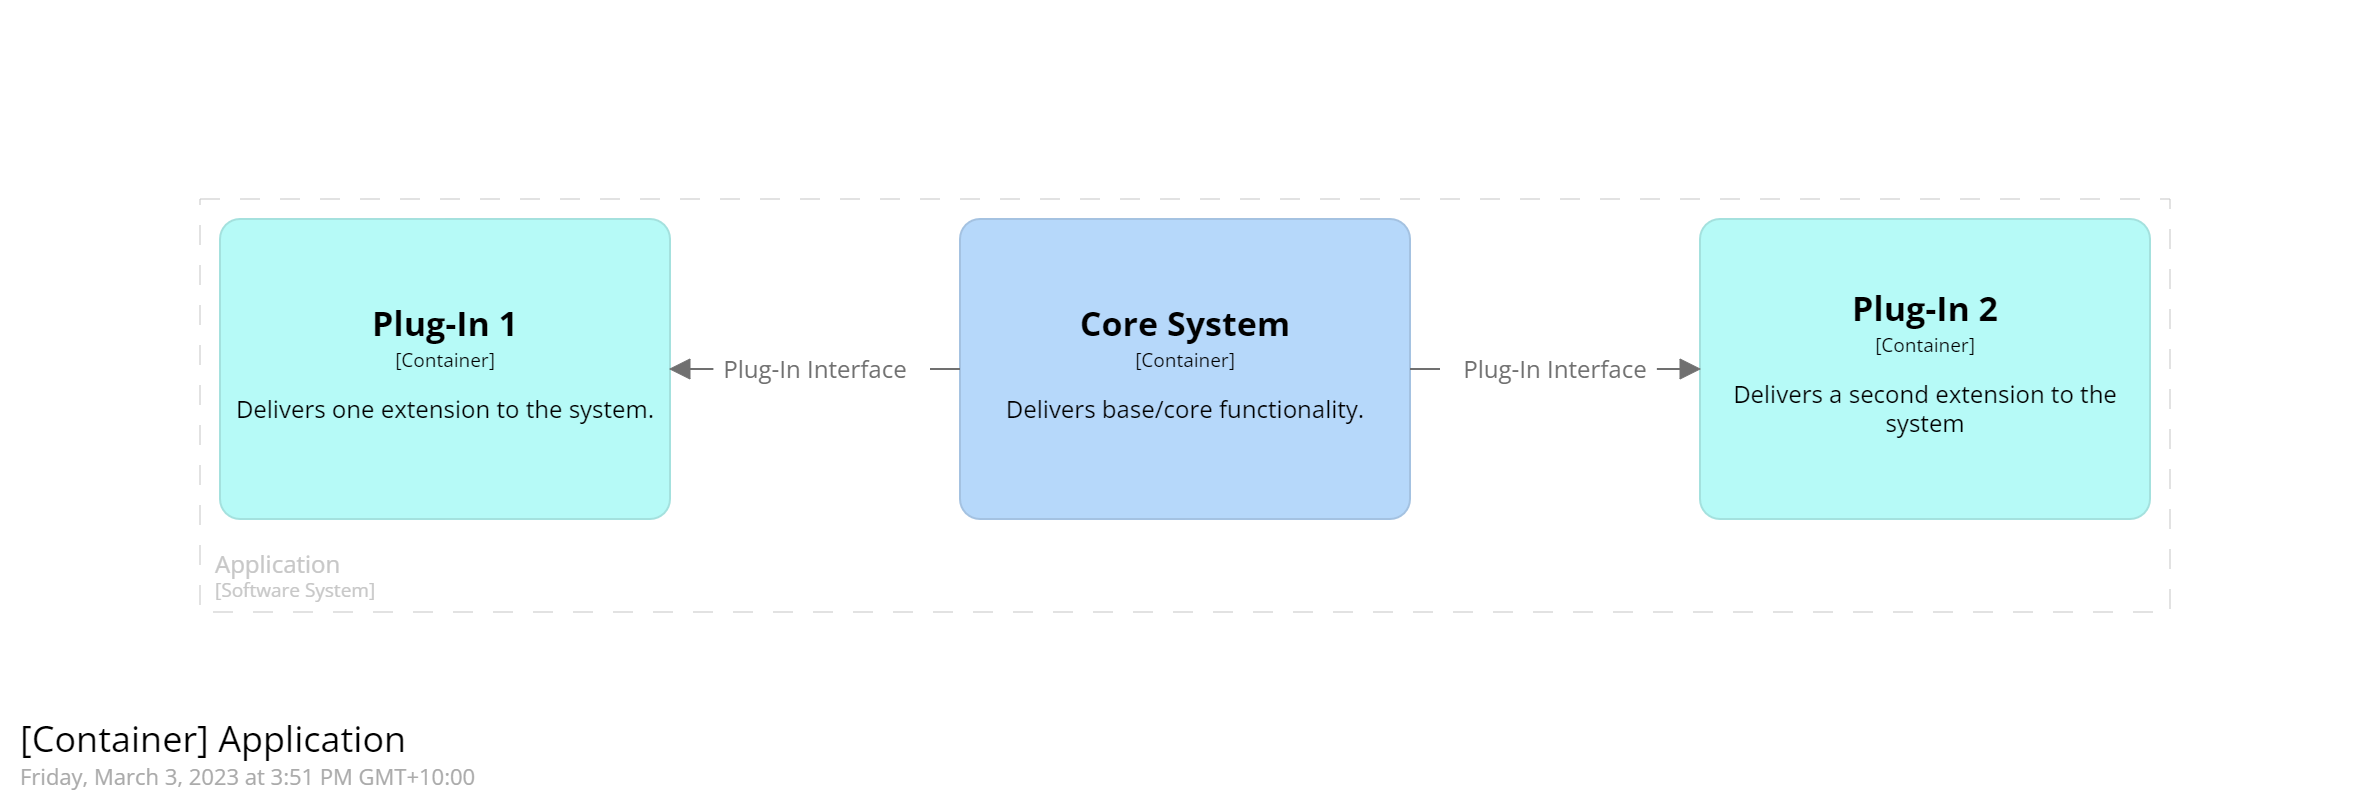
\includegraphics[trim=195 195 195 195,clip,width=0.85\textwidth]{diagrams/generic-microkernel.png}
    \caption{Generic structure of the microkernel architecture.}
    \label{fig:microkernel}
\end{figure}

For example, a web browser provides the core behaviour of rendering web pages.
Plug-ins extend the browser with specialised behaviour, such as a PDF viewer or dark mode reader.


\section{Terminology}

The microkernel architecture consists of four elements.
The \emph{core system}, \emph{plug-ins} and \emph{plug-in interface} shown in figure \ref{fig:microkernel}, plus a \emph{registry}.

\begin{description}
    \item[Core system] implements the system's base functionality.
    \item[Plug-ins] extend the system by providing independent, specialised behaviour.
    \item[Plug-in interface] describes how the core system and plug-ins interact.
    \item[Registry] tracks which plug-ins are available to the core system and how to access them.
\end{description}

The core system implements the minimal functionality that provides the base, or framework, of the system.
This may be the core functionality of the system, like the Eclipse editor or a web browser's page rendering engine.
Alternatively, the core system may implement a general processing path, like a payroll system's payment process.

The payment process may be simply, identify an employee, calculate their fortnightly pay, and send payment to their bank account.
Calculating pay can be a very complex process\footnote{\raggedright See the Queensland Health payroll disaster
\url{https://www.henricodolfing.com/2019/12/project-failure-case-study-queensland-health.html}}.
There are different pay rates, bonuses, incentives, salaried staff, staff paid commission, staff paid hourly rates,
overtime rates, penalty rates, deductions, taxes, and many other pay related calculations to consider for each individual.

Plug-ins are independent components that extend the behaviour of the core system.
The simple approach is that the system is delivered as a monolith, including the core system and the plug-ins.
In this case the core system uses the plug-ins via a method invocation.

In the payroll example, plug-ins can remove the complexity of different pay adjustment calculations from the core system
by moving each calculation to a separate component.
This also improves extensibility, maintainability and testability of the system.
New calculations can be added to the system by implementing new plug-ins.
As each plug-in is independent of the others, it is easier to implement a new calculation, or change an existing one,
than trying to do so in a large monolith.
New plug-ins can be tested independently and then integrated into the system for system testing.

There is usually a single standard interface between the core system and the plug-ins for a domain.
The interface defines the methods that the core system can invoke, data passed to the plug-in, and data returned from the plug-in.
A plug-in component implements the interface and delegates responsibilities within the component to deliver its behaviour.

Figure \ref{fig:interface} is an example of a possible interface for the pay adjusment calculation plug-ins.
Each pay adjustment plug-in returns a \texttt{MonetaryAmount} indicating the amount by which the employee's base pay is to be adjusted in the pay period.
The amount may be positive or negative.
The \texttt{employee}, \texttt{periodDetails}, \texttt{employeeConditions} and \texttt{basePay} objects are passed as parameters to the plug-in.
The plug-in can request the data it needs from these objects to perform its calculation.
The \texttt{periodDetails} object provides data about the work performed by the employee during the pay period (e.g. time worked, overtime, higher duties adjustments, ...).
The \texttt{employeeConditions} set provides data about each of the employee's pay conditions (e.g. before tax deductions, union membership, ...).

\begin{figure}[h]
\centering
\begin{shaded}
\begin{lstlisting}[style=java]
public interface PayAdjustmentPlugin {
    public MonetaryAmount adjustPay(Employee employee,
                                    WorkDetail periodDetails,
                                    Set<Condition> employeeConditions,
                                    MonetaryAmount basePay);
}
\end{lstlisting}
\end{shaded}
\caption{Example plug-in interface for payroll system.}
\label{fig:interface}
\end{figure}

The registery records which plug-ins are available to the core system and how they are accessed.
For the simple case of plug-ins being used by method invocation,
the registry just needs to record the name of the plug-in and a reference to the object that implements the plug-in's interface.
For the payroll example, this could be a simple map data structure.
The core system could lookup a plug-in by its name and then apply it by invoking the \texttt{adjustPay} method on the plug-in object.

\section{Microkernel Principles}
While the concept of a microkernel architecture is straightforward,
there are some principles which should be maintained to produce a maintainable and extendable architecture.

\begin{definition}[Independent Plug-in Principle]\label{independent-plug-in}
    Plug-ins should be independent, with no dependencies on other plug-ins.
    The only dependency on the core system is through the plug-in interface.
\end{definition}

Plug-ins should be independent of each other.
If a plug-in depends on other plug-ins it increases the complexity of the design.
This complexity is called \link{\emph{coupling}}{https://leanpub.com/isaqbglossary/read\#term-coupling},
which is a measure of how dependent different parts of a system are on each other \cite{glossary-architecture}.
High coupling (many dependencies) makes it difficult to understand the software,
which in turn makes it difficult to modify and test the software.
Consequently, if a plug-in depends on other plug-ins it requires understanding the dependencies on the other plug-ins to modify or test the plug-in.
This can lead to an architecture that resembles a ``big ball of mud''.

Plug-ins and the core system should be \emph{loosely} coupled.
The core system should only depend on the plug-in interface and data returned via that interface, not any implementation details of individual plug-ins.
Plug-ins should only depend on the data passed to them via the plug-in interface.
Plug-ins should not rely on implementation details of the core system, nor its datastore.
If plug-ins and the core system are not isolated from each other by an interface,
then any changes to the core system may require changes to some or all of the plug-ins.
Similarly, the plug-in interface should mean that any changes to the plug-in will have no impact on the core system.

\vspace{1mm}
\begin{definition}[Standard Interface Principle]\label{std-intf}
    There should be a single interface that defines how the core system uses plug-ins.
\end{definition}

\begin{wrapfigure}{r}{0.24\textwidth}
    \vspace{-18pt}
    \centering
    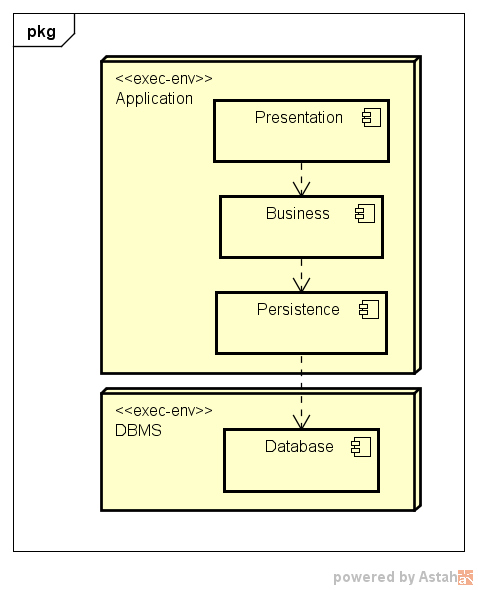
\includegraphics[trim=197 197 197 197,clip,width=0.24\textwidth]{diagrams/technical-partitioning.png}
    \vspace{-20pt}
    \caption{Layered architecture as example of technical partitioning.}
    \label{fig:technical-partitioning}
\end{wrapfigure}

To provide an extensible design, the core system needs a standard way to use plug-ins.
This means that the plug-in interface needs to be the same for all plug-ins.
That way the core system can use any plug-in without needing to know details about how the plug-in is implemented.
This again is about reducing coupling between the core system and the plug-ins.
The standard interface principle means that there is no additional complexity if the core system uses two plug-ins or two thousand plug-ins.


\section{Architecture Partitioning}

\subsection{Technical Partitioning}
The course notes about layered architecture \cite{layered-notes}
described the idea of partitioning an architecture into layers, as in figure \ref{fig:technical-partitioning}.

This approach to partitioning the architecture is called \emph{technical partitioning}.
Each layer represents a different technical capability.
The presentation layer deals with user interaction.
The business layer deals with the application's core logic.
The persistence layer deals with storing and loading data.
The database layer deals with file storage and access details.

\clearpage
An advantage of technical partitioning is that it corresponds to how developers view the code.
Another advantage is that all related code resides in a single layer of the architecture, making each layer
\link{cohesive}{https://leanpub.com/isaqbglossary/read\#term-cohesion} from a technical perspective.
This makes it easier to work with different parts of the code that deal with the same technical capability.
The \emph{layer isolation}, \emph{neighbour communication}, \emph{downward dependency},
and \emph{upward notification} principles help reduce coupling between layers.

A disadvantage of technical partitioning is that business processes cut across technical capabilities.
Consider when a customer adds a new product to their shopping cart in the Sahara eCommerce example
from the architectural views notes \cite{view-notes}.
In a technically partitioned architecture, code to implement this is required in all layers of the architecture.
If the team is structured with specialist developers who work on different layers of the architecture,
they all need to collaborate to implement the behaviour, which adds communication overheads to the project.

Another disadvantage is the potential for higher data coupling, if all domain data is stored in a single database.
If it is decided that the system needs to be split into distributed software containers for scalability,
the database may need to be split to have separate databases for each distributed container.
If the database was originally designed to cater for a monolith architecture, large parts of the database may need to be refactored.

Note that in figure \ref{fig:technical-partitioning}, and most of the following figures,
deployment nodes are used to explicitly indicate where components are executing in different environments.

\subsection{Domain Partitioning}
\emph{Domain partitioning} is an alternative approach, where the architecture is split into partitions (or major components)
corresponding to independent business processes or workflows (the \emph{domains}).
The implementation of a domain is responsible for delivering all of that workflow's behaviour.
Eric Evans popularised domain partitioning in his book \textit{Domain-Driven Design} \cite{ddd-evans}.
Figure \ref{fig:domain-partitioning} is an example of domain partitioning for an on-line store, similar to the
Sahara eCommerce example from the architectural views notes \cite{view-notes}.

\begin{figure}[h!]
    \centering
    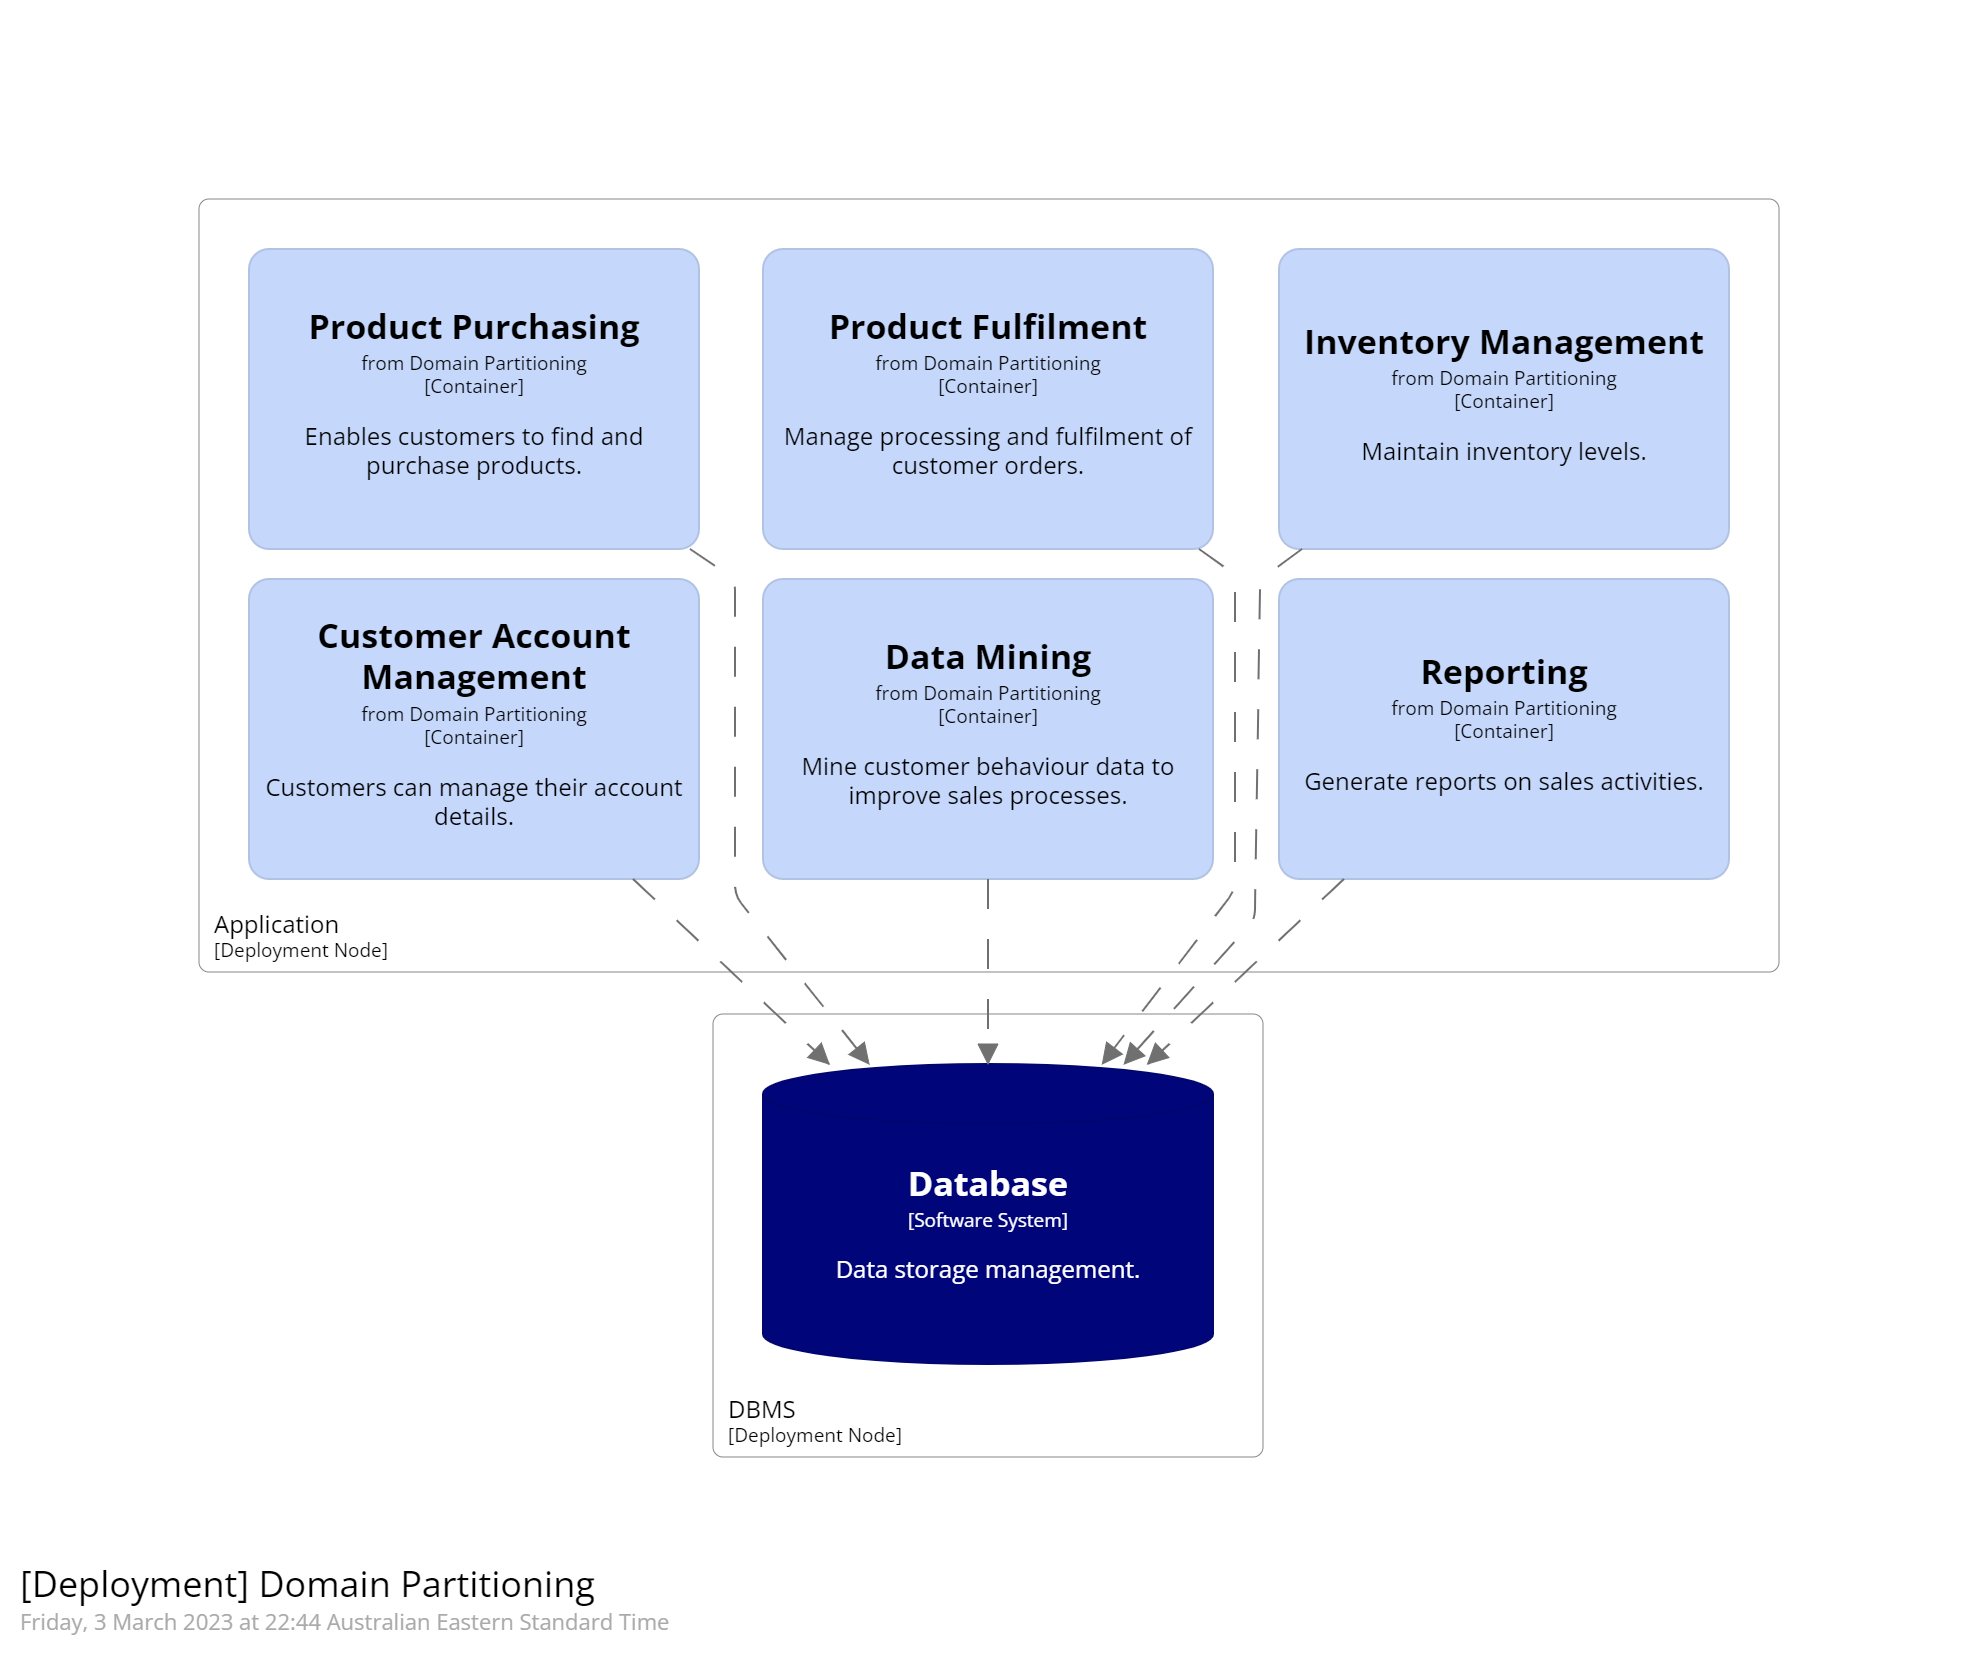
\includegraphics[trim=38 42 19 44,clip,width=0.9\textwidth]{diagrams/domain-partitioning.png}
    \caption{Example of domain partitioning.}
    \label{fig:domain-partitioning}
\end{figure}

An advantage of domain partitioning is that it can model how the business functions, rather than it being structured based on technical decisions.
This results in message flows within the software matching how communication happens in the problem domain.
This makes it easier to discuss features, and the high-level view of how they are implemented, with business stakeholders who are familiar with how the business operates.

If the domain partitions are independent of each other, it usually makes it easier to split the system into distributed software containers.
Even if the system starts with a single database, the independence of domain partitions is likely to lead to a design with lower data coupling,
making it easier to split the database.

Another advantage of domain partitioning is that it fits well with an agile or continuous delivery process.
A single user story will be implemented entirely within one domain.
This also makes it easier to implement multiple user stories concurrently, if they are all from different domains.

A disadvantage of domain partitioning is that \emph{boundary} code is distributed throughout all the partitions.
This means that any large changes to a particular boundary (e.g. changing the persistence library) will result in changes to all domain partitions.
Boundary code is code that interacts with actors or agents outside of the system.
The two common technical partitions of the presentation and persistence layers are examples of boundary code.
The presentation layer is the boundary between the system and the users.
The persistence layer is the boundary between the system and the storage mechanisms.
Other boundary partitions may be for message queues or network communication.

It is possible for each domain partition to use technical partitioning within it,
to provide some of the lower coupling benefits of a layered architecture for the domain.

\subsection{Achitecture Patterns and Partitioning}
Different architecture patterns are biased more towards technical or domain partitioning.
Those that focus on technical structure are biased towards technical partitioning (e.g. layered architecture).
Those that focus on message passing between components are biased towards domain partitioning (e.g. microservices architecture).
The core system of the microkernel architecture can follow either technical or domain partitioning.

A consequence of this leads to a variation of principle \ref{std-intf}.

\vspace{1mm}
\begin{definition}[Domain Standard Interface Principle]\label{domain-intf}
    Each \emph{domain} should have a single interface that defines how the domain uses plug-ins.
\end{definition}

Some domains may share a plug-in interface, but allowing domains to have different plug-in interfaces
means that each business process can be customised independently by a set of plug-ins.

\begin{figure}[h!]
    \centering
    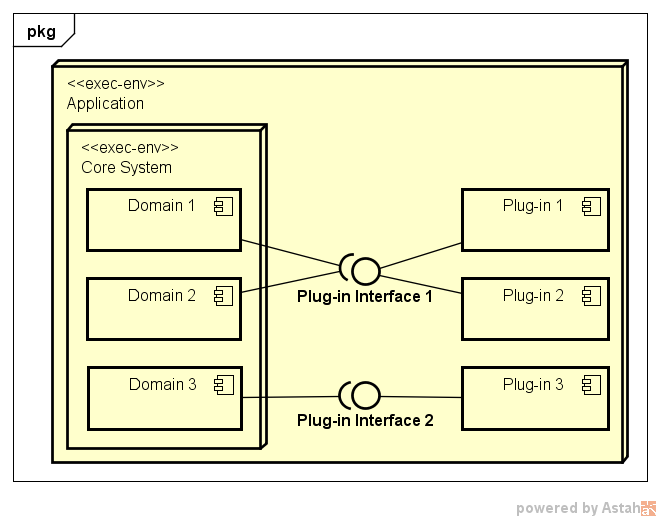
\includegraphics[trim=38 42 23 42,clip,width=0.5\textwidth]{diagrams/domain-microkernel.png}
    \caption{Microkernel architecture with domains.}
    \label{fig:microkernel-domains}
\end{figure}

In figure \ref{fig:microkernel-domains}, nodes are used to explicitly indicate that the core system and plug-ins are conceptually separate from each other.
They are all contained within the Application node to indicate that they are still all part of one monolithic application.


\section{Extensions}

While the microkernel architecture often implements the core system as a monolith
and it, along with all its plug-ins, is often deployed as a single monolith
(e.g. a web browser), that is not the only approach to using the microkernel architecture.

\subsection{Distributed Microkernel}

The internal partitions of the core system can be distributed to run on different computing infrastructure.
Figure \ref{fig:3-tier-microkernel} is an example of implementing a distributed microkernel architecture using three computing tiers.

\begin{figure}[h!]
    \centering
    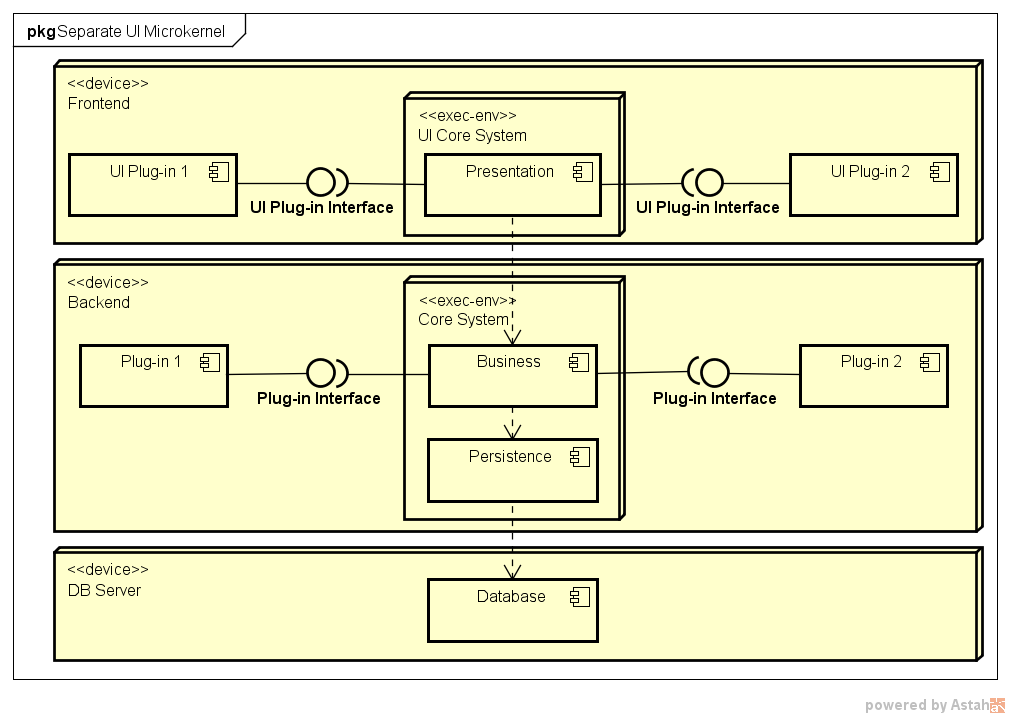
\includegraphics[trim=40 41 18 43,clip,width=0.9\textwidth]{diagrams/separate-ui-microkernel.png}
    \caption{Microkernel architecture distributed by technical partitions.}
    \label{fig:3-tier-microkernel}
\end{figure}

The presentation layer runs on a frontend such as a web or mobile application.
It is possible that the presentation layer could have its own set of plug-ins.
The business and persistence logic run on a backend server and have their own set of plug-ins.
The database runs on a separate database server, and typically does not have any plug-ins from the application's perspective.

\subsection{Alternative Contracts}

Figure \ref{fig:interface} was an example interface that could be used if plug-ins were invoked directly within the core system.
This is possible if the plug-ins are implemented within the application or are loaded as code modules at run time (e.g. via JAR or DLL files).

There may be times when plug-ins are external services used by the core system.
In those situations communication is via some communication protocol.
Remote method invocation would still allow the core system to use a compiled interface.
Registration of components would become a little more complicated,
as the core system would need to a communication interface to be notified of the availability of plug-ins.

More commonly, the communication protocol will be some other mechanism (e.g. REST, as shown in figure \ref{fig:rest-microkernel}).
In this case, the registry needs to record more information than just the name and interface of a plug-in.
The registry will need information about the communication pathway (e.g. URL of the REST endpoint).
It will also need details about the data structure passed to the plug-in and returned by the plug-in.

\begin{figure}[h!]
    \centering
    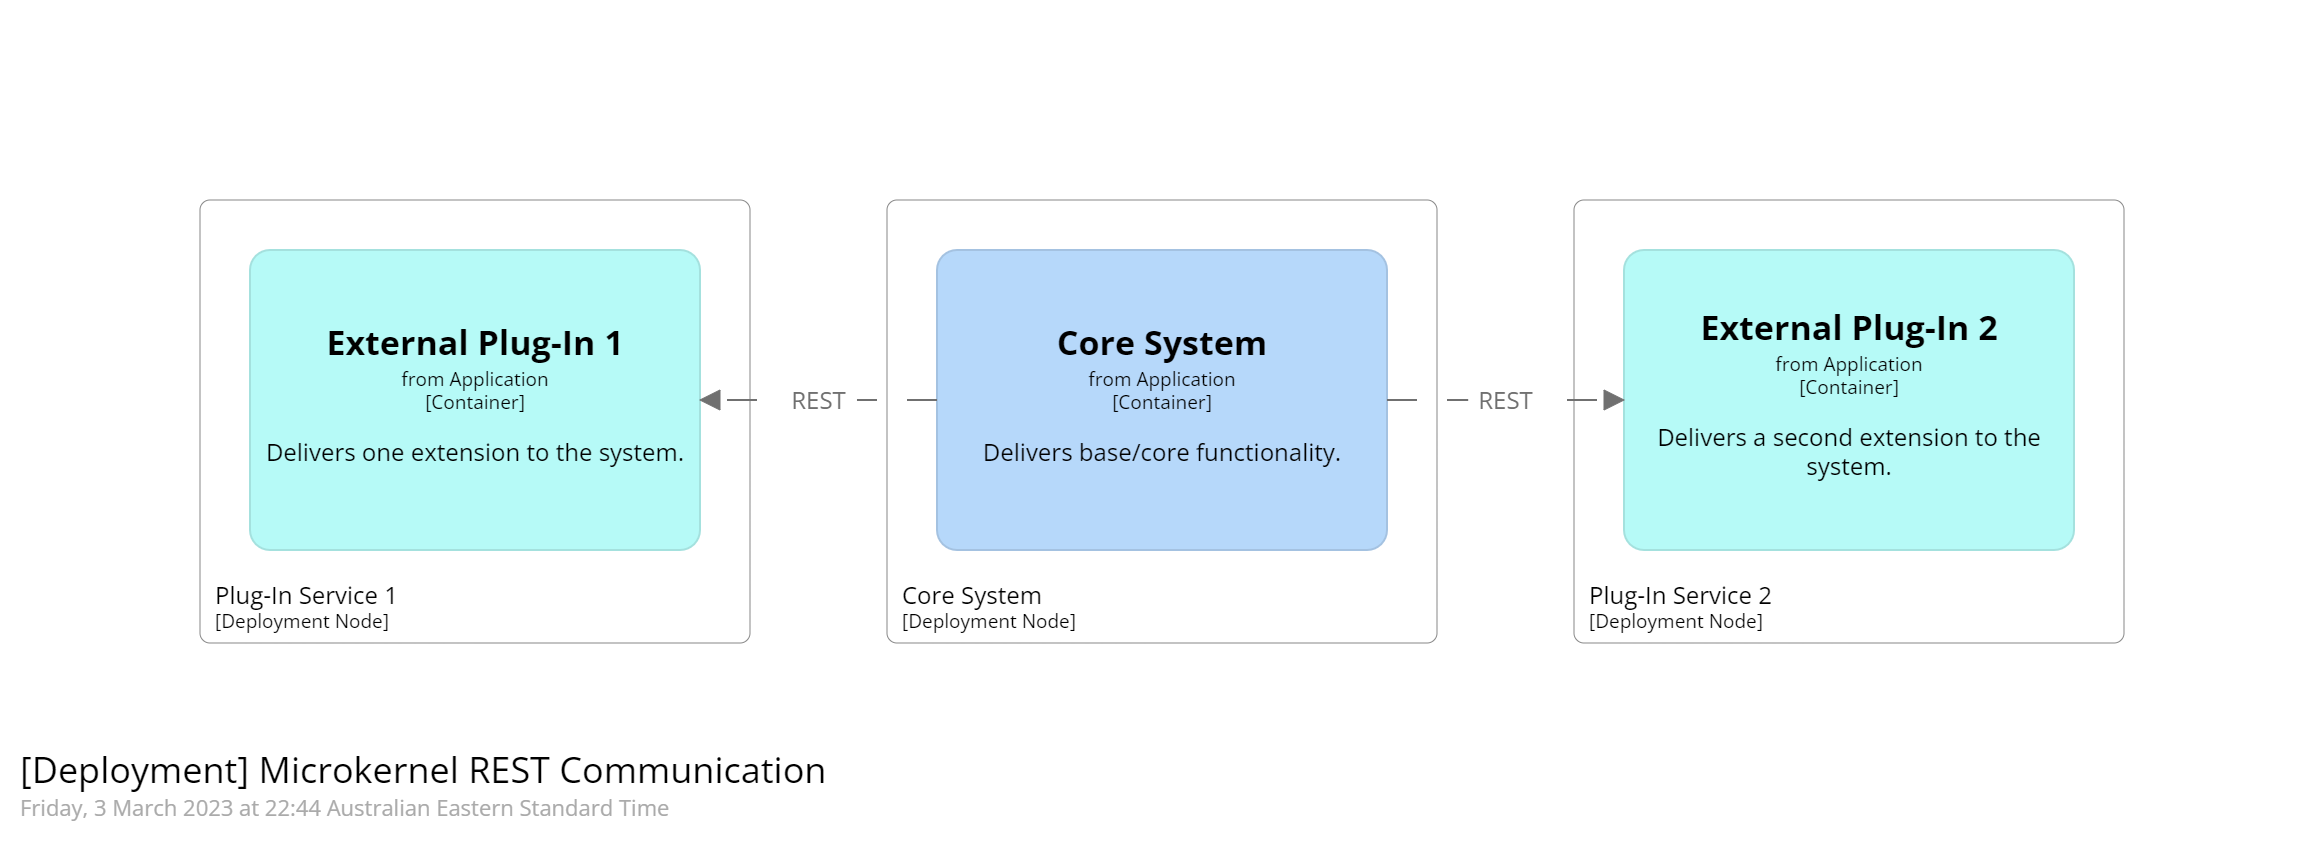
\includegraphics[trim=38 167 19 45,clip,width=0.75\textwidth]{diagrams/rest-microkernel.png}
    \caption{Microkernel architecture -- separate plug-in services with REST communication.}
    \label{fig:rest-microkernel}
\end{figure}

\subsection{Plug-in Databases}

As mentioned in the discussion of principle \ref{independent-plug-in}, plug-ins should not use the core system's data directly.
The core system should pass to the plug-in any data that it needs.
For sophisticated plug-ins, they may need their own persistent storage.
They should not request the core system to manage this.
Rather, these plug-ins should maintain their own databases, as shown in figure \ref{fig:plug-in-dbs}.

\begin{figure}[h!]
    \centering
    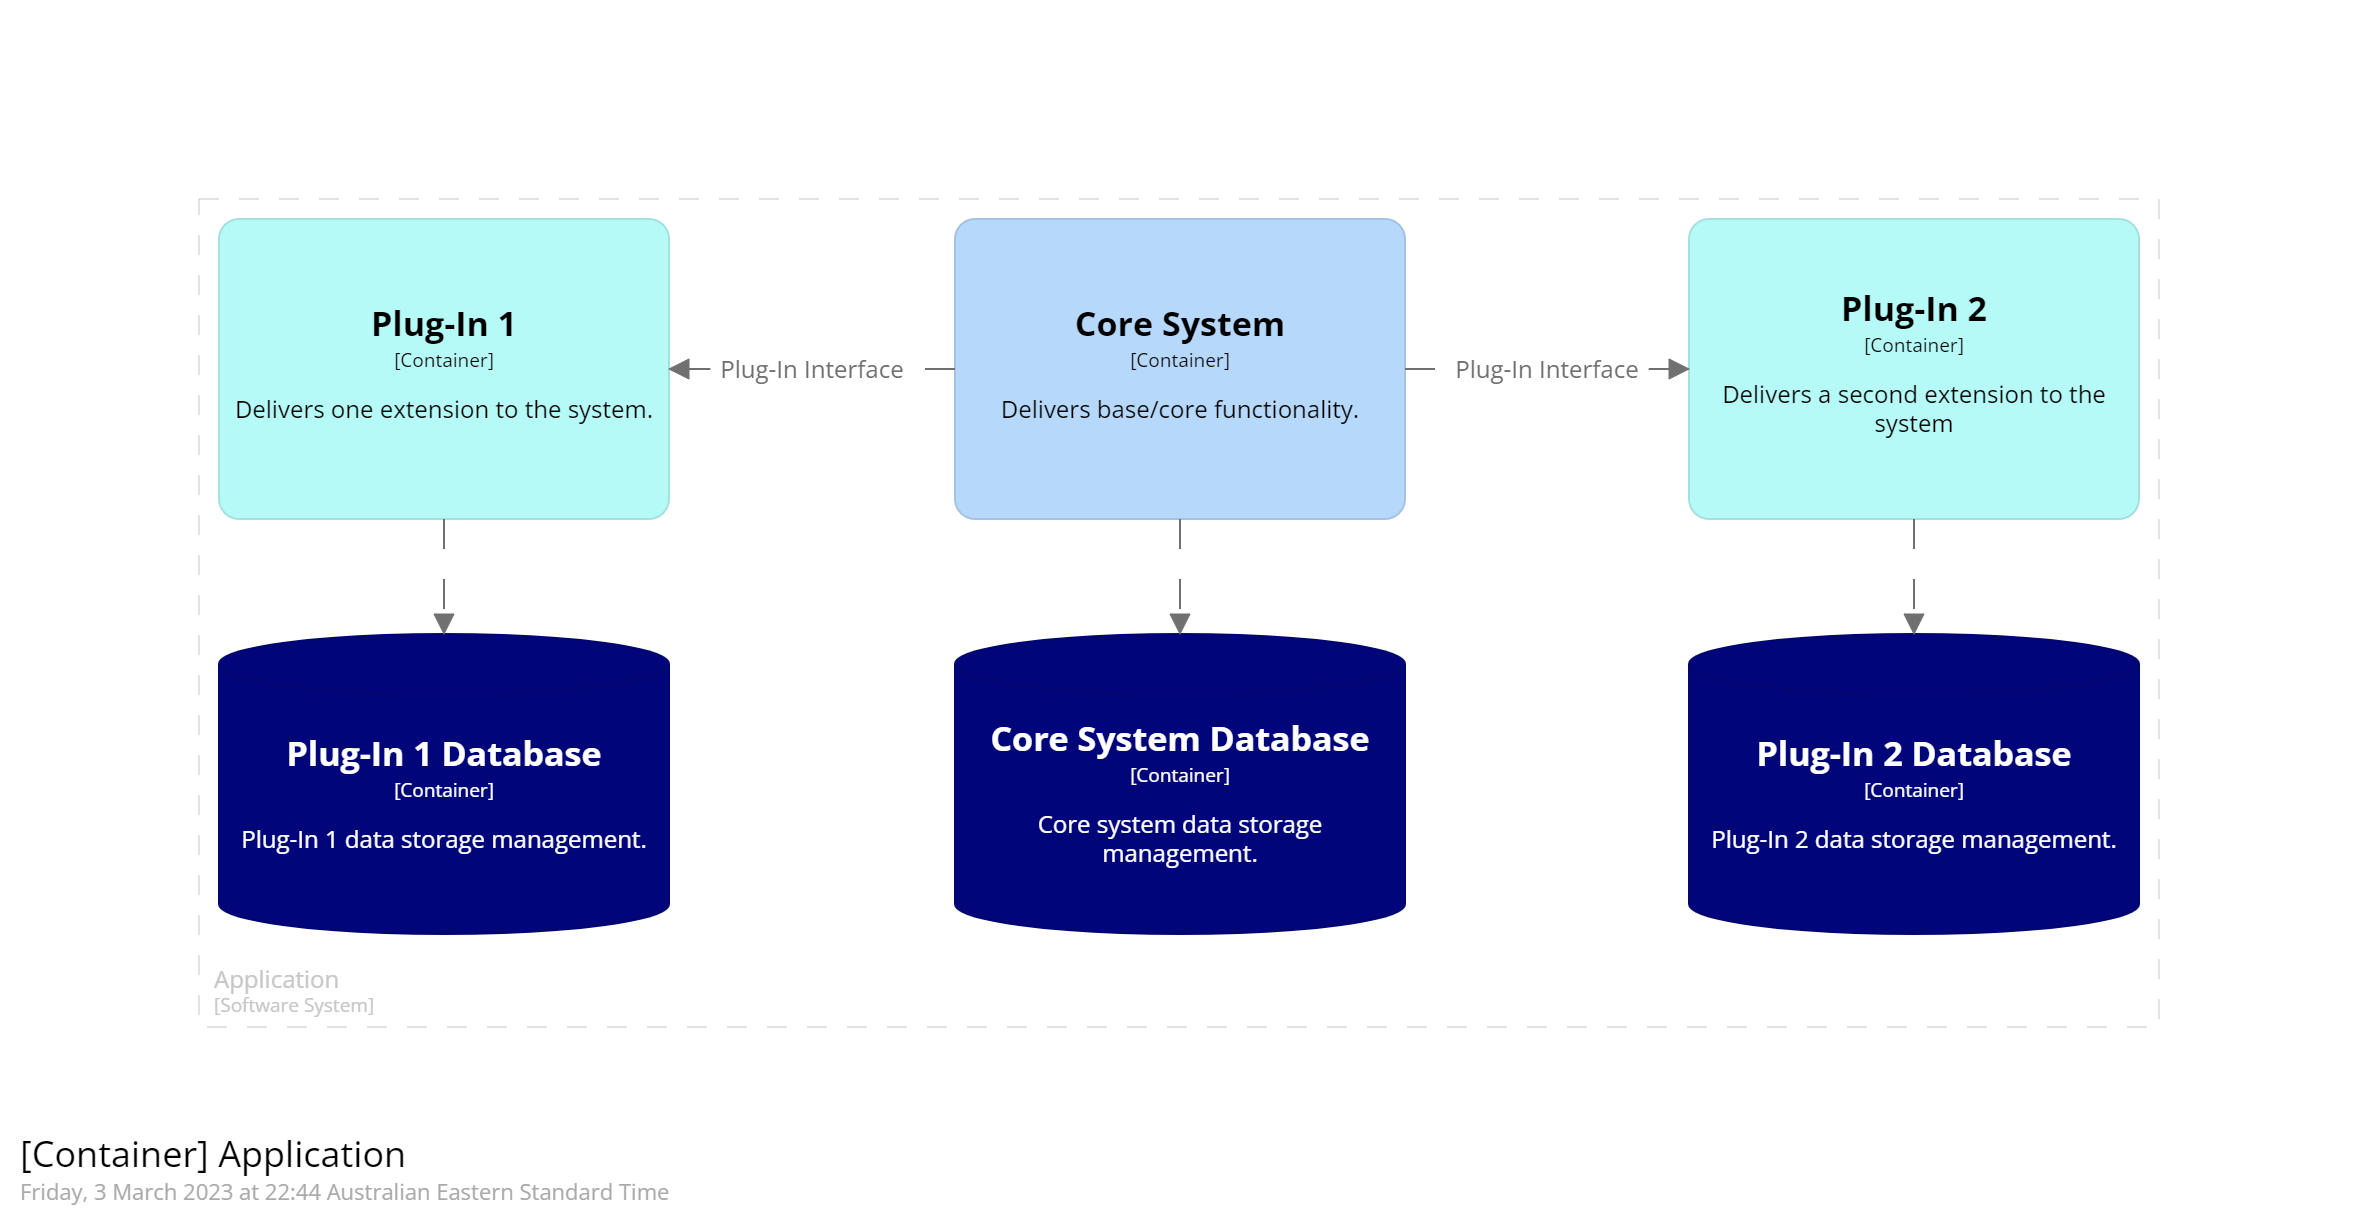
\includegraphics[trim=38 81 24 50,clip,width=0.85\textwidth]{diagrams/plug-in-databases.png}
    \caption{Microkernel architecture with plug-ins maintaining their own databases.}
    \label{fig:plug-in-dbs}
\end{figure}

\subsection{Non-Standard Interfaces}

Principles \ref{std-intf} and \ref{domain-intf} indicate that each domain, or the entire core system, should use a single plug-in interface.
This is not always possible when the plug-ins are services provided by external agencies.
In these situations you would use the \link{adapter design pattern}{https://refactoring.guru/design-patterns/adapter}
to isolate the external service's interface from the core system.

\begin{figure}[h!]
    \centering
    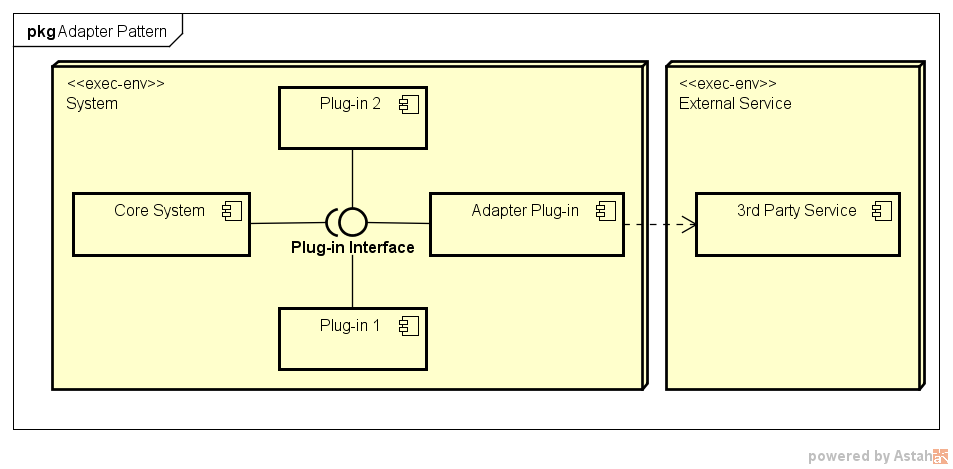
\includegraphics[trim=38 58 20 45,clip,width=0.85\textwidth]{diagrams/adapter-plug-in.png}
    \caption{Adapter plug-ins to work with third party services.}
    \label{fig:adapter}
\end{figure}

As shown in figure \ref{fig:adapter}, an adapter plug-in is implemented that manages communication with the external service.
From the core system's perspective, the external system is just like any other plug-in.


\section{Conclusion}

The microkernel architecture is a suitable option for systems were extensibility is a key quality attribute.
Following the microkernel design principles will lead to a design where the core system and plug-ins are not affected by changes to each other.
Existing plug-ins can be replaced and new plug-ins added with no impact on the core system.
